\documentclass[conference]{IEEEtran}
\usepackage[utf8]{inputenc}
\usepackage[T1]{fontenc}
\usepackage[french]{babel}
\usepackage{amsmath,amssymb}
\usepackage{graphicx}
\usepackage{booktabs}
\usepackage{tikz}
\usetikzlibrary{arrows.meta,positioning,shapes.geometric,shapes.multipart,fit,calc}
\usepackage[hidelinks]{hyperref}



\begin{document}

\title{Algorithme d'\'Evolution Diff\'erentielle massivement parall\`ele sur GPU avec CUDA : comparaison avec la version s\'equentielle}

\author{
  \IEEEauthorblockN{Zainab Elamri, Omar Elsemry, Mohamed De Franceschi}
  \IEEEauthorblockA{Master IM -- Universit\'e de Haute-Alsace (UHA)\\
  Enseignant : Lhassane IDOUMGHAR}
}

\maketitle

\begin{abstract}
\textit{[\`A compl\'eter]}
\end{abstract}

\begin{IEEEkeywords}
Differential Evolution, GPU, CUDA, massively parallel metaheuristics, global optimization, benchmark functions.
\end{IEEEkeywords}

\section{Introduction}
\textit{[\`A compl\'eter]}

\section{Programmation GPU}
\textit{[\`A compl\'eter]}

\section{\'Evolution Diff\'erentielle}
\subsection{Aper\c cu de la version s\'equentielle}
\textit{[\`A compl\'eter]}

\subsection{Description de la version massivement parall\`ele}
\textit{[\`A compl\'eter]}

% ---------- Organigramme (style de l'article) ----------
\begin{figure}[!t]
\centering
\begin{tikzpicture}[font=\fontsize{6}{7}\selectfont,>={Stealth[length=1.5mm]},x=1cm,y=1cm,
  hb/.style={draw,rounded corners=4pt,align=center,minimum width=2.1cm,minimum height=0.55cm,inner sep=1pt},
  kb/.style={draw,align=center,minimum width=3.1cm,minimum height=0.6cm,inner sep=1pt},
  rw/.style={font=\fontsize{5}{6}\selectfont\bfseries}]
  % en-t\^etes
  \node[font=\fontsize{6}{7}\selectfont\bfseries,align=center] at (1.2,0.35) {CPU (h\^ote)\\1 thread};
  \node[font=\fontsize{6}{7}\selectfont\bfseries,align=center] at (4.9,0.35) {GPU (device)\\\textit{gridDim $\times$ blockDim threads}};
  \draw[dashed,gray] (2.75,0.8) -- (2.75,-7.4);
  % barre m\'emoire globale
  \node[draw,fill=gray!25,minimum width=0.4cm,minimum height=6.2cm,inner sep=0] (gm) at (7.9,-3.4) {};
  \node[rotate=-90,font=\fontsize{6}{7}\selectfont\bfseries] at (7.9,-3.4) {M\'emoire globale};
  % h\^ote
  \node[hb] (init) at (1.2,-0.7) {Allocation m\'emoire\\Copie H$\to$D};
  \node[draw,diamond,aspect=2.4,inner sep=0pt,align=center] (dec) at (1.2,-4.3) {g\'en\'eration\\$<$ maxGen ?};
  \node[hb] (ret) at (1.2,-6.6) {Retourner le\\meilleur individu};
  % noyaux
  \node[kb] (ki) at (4.9,-1.4) {\textbf{kernel (I)}\\[-1pt]\textcolor{gray}{kernelInitRandom}};
  \node[kb] (ke) at (4.9,-2.9) {\textbf{kernel (E)}\\[-1pt]\textcolor{gray}{kernelEvaluate}};
  \node[kb,minimum height=1.5cm] (kg) at (4.9,-4.9) {\textbf{kernel (G)}\\[-1pt]\textcolor{gray}{kernelDEGeneration :}\\[-1pt]\textcolor{gray}{mutation, croisement,}\\[-1pt]\textcolor{gray}{\'evaluation, s\'election}};
  % fl\`eches h\^ote -> noyaux
  \draw[->] (init.south) -- ++(0,-0.35) -| node[pos=0.25,above,rw]{kernel call} (ki.west);
  \draw[->] (init.south)++(0,-0.35) -- ++(0,0) ;
  \draw[->] (1.2,-1.05) |- node[pos=0.8,above,rw]{kernel call} (ke.west);
  \draw[->] (1.2,-2.9) -- (dec.north);
  \draw[->] (dec.east) -- node[above,rw]{oui} node[below,rw]{kernel call} (kg.west |- dec.east);
  \draw[->] (dec.south) -- node[right,rw]{non} (ret.north);
  % boucle de retour
  \draw[->] (kg.south) -- ++(0,-0.35) -| (2.45,-3.55) -- (1.2,-3.55);
  % lectures / \'ecritures m\'emoire
  \foreach \k/\yy in {ki/-1.4,ke/-2.9,kg/-4.9}{
    \draw[<-] ($(\k.east)+(0,0.12)$) -- node[above,rw]{read} ($(gm.west |- \k.east)+(0,0.12)$);
    \draw[->] ($(\k.east)+(0,-0.12)$) -- node[below,rw]{write} ($(gm.west |- \k.east)+(0,-0.12)$);
  }
\end{tikzpicture}
\caption{Organigramme du DE massivement parall\`ele (un thread par individu).}
\label{fig:sequence}
\end{figure}

\section{R\'esultats exp\'erimentaux}
\subsection{Configuration}
\textit{[\`A compl\'eter]}

\subsection{Fonctions de test}
\textit{[\`A compl\'eter]}

\subsection{R\'esultats}
\begin{figure}[!t]
\centering
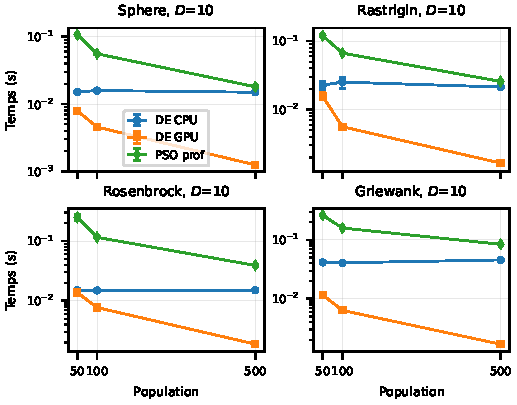
\includegraphics[width=\columnwidth]{figures/temps_d10.pdf}
\caption{Temps d'ex\'ecution moyen (\'echelle logarithmique) en fonction de la population, $D=10$ (barres : \'ecart-type sur 10 runs).}
\label{fig:temps10}
\end{figure}

\begin{figure}[!t]
\centering
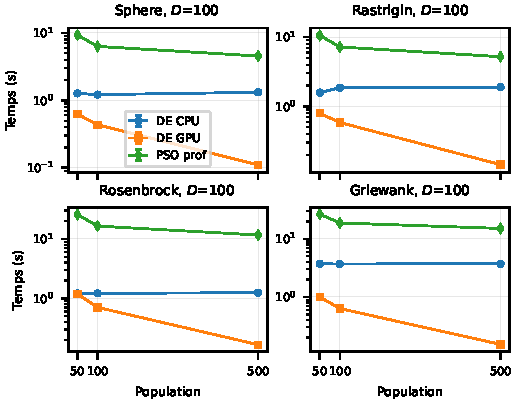
\includegraphics[width=\columnwidth]{figures/temps_d100.pdf}
\caption{Temps d'ex\'ecution moyen en fonction de la population, $D=100$.}
\label{fig:temps}
\end{figure}

\begin{table}[!t]\centering\scriptsize\setlength{\tabcolsep}{2pt}\caption{Temps moyen (s) sur les 4 fonctions (40 runs par case).}\label{tab:temps}
\begin{tabular}{rr|ccc}\toprule Dim & Pop & DE CPU & DE GPU & PSO prof\\\midrule
10 & 50 & 0.024 & 0.012 & 0.185\\
10 & 100 & 0.024 & 0.006 & 0.099\\
10 & 500 & 0.024 & 0.002 & 0.042\\
\midrule
50 & 50 & 0.478 & 0.389 & 4.567\\
50 & 100 & 0.499 & 0.222 & 3.071\\
50 & 500 & 0.502 & 0.052 & 2.092\\
\midrule
100 & 50 & 1.945 & 0.902 & 18.047\\
100 & 100 & 1.996 & 0.589 & 12.201\\
100 & 500 & 2.046 & 0.143 & 9.128\\
\bottomrule\end{tabular}\end{table}

\begin{table}[!t]\centering\scriptsize\setlength{\tabcolsep}{2pt}\caption{Taux de succ\`es, forme \emph{article / DE GPU $CR{=}0{,}9$ / DE GPU $CR{=}0{,}3$}. Article \cite{qin} : EFV $<10^{-8}$, 25 runs ; nos valeurs : EFV $<10^{-4}$, 10 runs.}\label{tab:sr}
\begin{tabular}{lr|ccc}\toprule Fonction & Dim & Pop 50 & Pop 100 & Pop 500\\\midrule
Sphere & 10 & 1.00/1.00/1.00 & 1.00/1.00/1.00 & 1.00/1.00/1.00\\
Sphere & 50 & 1.00/1.00/1.00 & 1.00/1.00/1.00 & 1.00/0.00/1.00\\
Sphere & 100 & 1.00/1.00/1.00 & 1.00/1.00/1.00 & 1.00/0.00/0.00\\
Rastrigin & 10 & 1.00/0.50/1.00 & 1.00/0.00/1.00 & 1.00/0.00/0.00\\
Rastrigin & 50 & 0.00/0.00/0.00 & 0.04/0.00/0.00 & 0.04/0.00/0.00\\
Rastrigin & 100 & 0.00/0.00/0.00 & 0.00/0.00/0.00 & 0.00/0.00/0.00\\
Rosenbrock & 10 & 0.44/0.00/0.00 & 0.32/1.00/0.00 & 0.00/0.00/0.00\\
Rosenbrock & 50 & 0.00/0.00/0.00 & 0.04/0.00/0.00 & 0.00/0.00/0.00\\
Rosenbrock & 100 & 0.00/0.00/0.00 & 0.00/0.00/0.00 & 0.00/0.00/0.00\\
Griewank & 10 & 1.00/0.20/0.90 & 1.00/0.80/1.00 & 1.00/0.00/0.00\\
Griewank & 50 & 0.92/1.00/1.00 & 1.00/1.00/1.00 & 1.00/0.00/1.00\\
Griewank & 100 & 0.84/0.90/1.00 & 0.96/1.00/1.00 & 0.96/0.00/1.00\\
\bottomrule\end{tabular}\end{table}


\section{Conclusion}
\textit{[\`A compl\'eter]}

\nocite{*}
\begin{thebibliography}{1}
\bibitem{qin} A.~K. Qin, F.~Raimondo, F.~Forbes, and Y.~S. Ong, ``An improved CUDA-based implementation of differential evolution on GPU,'' in \emph{Proc. GECCO'12}, Philadelphia, USA, 2012.
\end{thebibliography}

\end{document}
